\documentclass[a4paper, 10pt]{article}
\usepackage{scrextend}
\changefontsizes{9pt}
% Per-subject config for this repo. See vendor/template/course-config.tex.example
% for what each macro is used for.

\newcommand{\CourseCode}{2110473}
\newcommand{\CourseName}{Fault Tolerant Computing}
\newcommand{\StudentID}{6733172621}
\newcommand{\StudentName}{Patthadon Phengpinij}
\newcommand{\DefaultCollaborators}{Claude (for\,\LaTeX\,styling and grammar checking)}
\newcommand{\AssignmentLabel}{Homework}

\usepackage{../vendor/template/CEDT-Assignment-style}

\begin{document}
\subject
\asgntitle{11}{}{Week 13}{\StudentID\ \StudentName}{\DefaultCollaborators}

% ================================================================================ %
\section{Asynchronous Circuit Testing}
% ================================================================================ %

% ================================================================================ %
%                                    Problem 01                                    %
% ================================================================================ %
\begin{problem}
Show and explain a \textbf{\textit{\textcolor{red}{Late detection stuck-at-fault}}} in Dual-rail asynchronous One-bit Full Adder Circuit below.

\begin{table}[htbp]
	\centering
	\begin{minipage}[c]{0.48\linewidth}
		\centering
		\renewcommand{\arraystretch}{1.4}
		\setlength{\tabcolsep}{8pt}

		\begin{tabular}{|c|c|c|c|c|}
			\hline
			\footnotesize\shortstack{ \\Input\\bit for\\number\\$A$}
			  &
			\footnotesize\shortstack{ \\Input\\bit for\\number\\$B$}
			  &
			\footnotesize\shortstack{ \\Carry\\bit\\input\\$C_{\mathrm{IN}}$}
			  &
			\footnotesize\shortstack{ \\Sum\\bit\\output\\$S$}
			  &
			\footnotesize\shortstack{ \\Carry\\bit\\output\\$C_{\mathrm{OUT}}$}
			\\
			\hline
			0 & 0 & 0 & 0 & 0         \\
			0 & 0 & 1 & 1 & 0         \\
			0 & 1 & 0 & 1 & 0         \\
			0 & 1 & 1 & 0 & 1         \\
			1 & 0 & 0 & 1 & 0         \\
			1 & 0 & 1 & 0 & 1         \\
			1 & 1 & 0 & 0 & 1         \\
			1 & 1 & 1 & 1 & 1         \\
			\hline
		\end{tabular}
		\caption{Truth table of a full adder}
		\label{tab:full-adder}
	\end{minipage}%
	\hfill
	\begin{minipage}[c]{0.48\linewidth}
		\centering
		\resizebox{\linewidth}{!}{%
			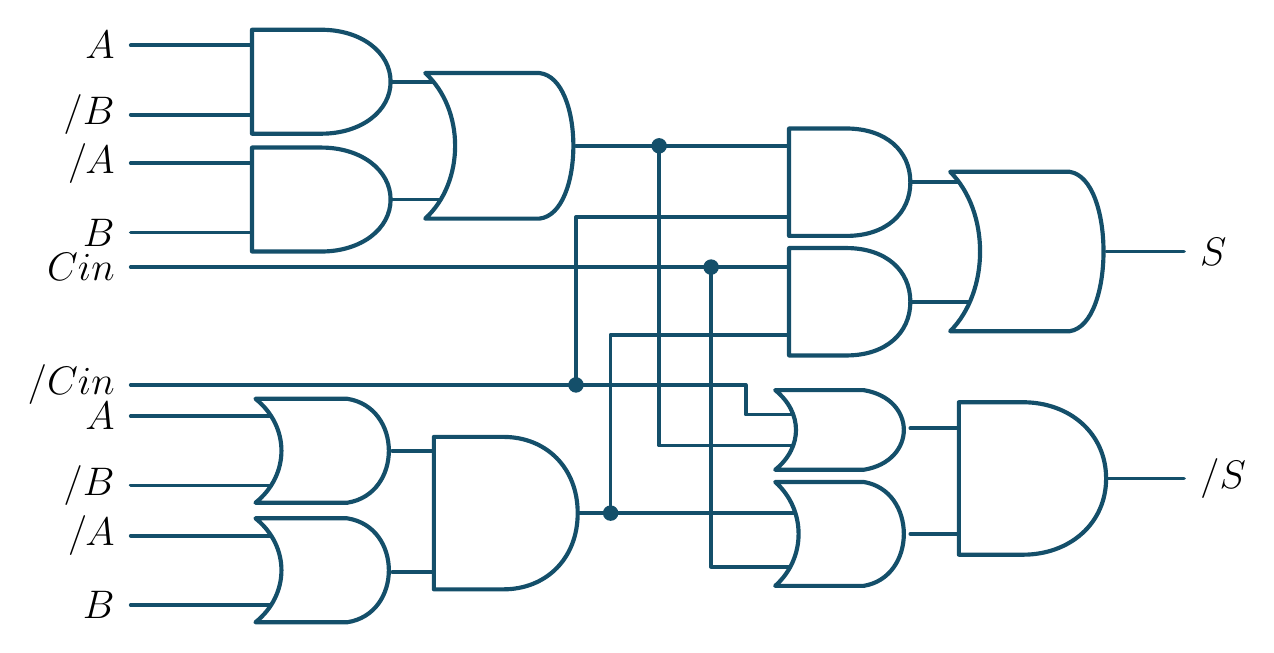
\begin{tikzpicture}[
					x=0.022cm,
					y=-0.022cm,
					wire/.style={
							draw=circuitblue,
							line width=1.35pt,
							line cap=round,
							line join=round
						},
					gate/.style={
							draw=circuitblue,
							fill=white,
							line width=1.5pt,
							line cap=round,
							line join=round
						},
					sig/.style={
							font=\Large,
							inner sep=0pt
						}
				]

				% =========================================================
				% Color
				% =========================================================
				\definecolor{circuitblue}{RGB}{20,79,106}

				% =========================================================
				% Upper input signals
				% =========================================================

				% A, /B
				\draw[wire] (65,55) -- (135,55);
				\draw[wire] (65,95) -- (135,95);

				% /A, B
				\draw[wire] (65,123) -- (135,123);
				\draw[wire] (65,163) -- (135,163);

				% Cin
				\draw[wire] (65,183) -- (445,183);

				% =========================================================
				% Lower input signals
				% =========================================================

				% /Cin: bend downward into upper lower-right OR
				% FIX: Input now enters the curved side at y = 268
				\draw[wire]
				(65,251) -- (420,251)
				-- (420,268) -- (457,268);

				% A, /B
				\draw[wire] (65,269) -- (157,269);
				\draw[wire] (65,309) -- (157,309);

				% /A, B
				\draw[wire] (65,338) -- (157,338);
				\draw[wire] (65,378) -- (157,378);

				% =========================================================
				% Upper-left AND outputs
				% =========================================================

				\draw[wire] (215,76) -- (258,76);
				\draw[wire] (215,144) -- (258,144);

				% =========================================================
				% Upper OR output and branches
				% =========================================================

				% OR -> upper AND
				\draw[wire]
				(322,113) -- (445,113);

				% Branch -> upper lower-right OR
				\draw[wire]
				(370,113) -- (370,286)
				-- (457,286);

				% =========================================================
				% /Cin branches
				% =========================================================

				% /Cin -> upper-right AND
				\draw[wire]
				(322,251) -- (322,154)
				-- (445,154);

				% =========================================================
				% Cin branches
				% =========================================================

				% Cin -> lower lower-right OR
				\draw[wire]
				(400,183) -- (400,356)
				-- (457,356);

				% =========================================================
				% Lower-left OR outputs
				% =========================================================

				\draw[wire]
				(216,289) -- (240,289);

				\draw[wire]
				(216,359) -- (240,359);

				% =========================================================
				% Lower-left AND output and branches
				% =========================================================

				% AND -> lower lower-right OR
				\draw[wire]
				(323,325) -- (457,325);

				% AND -> upper-right lower AND
				\draw[wire]
				(342,325) -- (342,222)
				-- (445,222);

				% =========================================================
				% Upper-right AND outputs
				% =========================================================

				\draw[wire]
				(515,134) -- (565,134);

				\draw[wire]
				(515,203) -- (565,203);

				% =========================================================
				% Lower-right OR outputs
				% =========================================================

				\draw[wire]
				(515,276) -- (543,276);

				\draw[wire]
				(515,337) -- (543,337);

				% =========================================================
				% Final output wires
				% =========================================================

				\draw[wire] (628,174) -- (673,174);
				\draw[wire] (628,305) -- (673,305);

				% =========================================================
				% Upper-left AND gate 1
				% =========================================================

				\draw[gate]
				(135,46) -- (175,46)
				.. controls (198,46) and (215,59) .. (215,76)
				.. controls (215,93) and (198,106) .. (175,106)
				-- (135,106) -- cycle;

				% =========================================================
				% Upper-left AND gate 2
				% =========================================================

				\draw[gate]
				(135,114) -- (175,114)
				.. controls (198,114) and (215,127) .. (215,144)
				.. controls (215,161) and (198,174) .. (175,174)
				-- (135,174) -- cycle;

				% =========================================================
				% Upper OR gate
				% =========================================================

				\draw[gate]
				(235,71)
				.. controls (259,71) and (288,71) .. (301,71)
				.. controls (327,74) and (327,152) .. (301,155)
				.. controls (288,155) and (259,155) .. (235,155)
				.. controls (258,134) and (258,92) .. (235,71)
				-- cycle;

				% =========================================================
				% Upper-right AND gate 1
				% =========================================================

				\draw[gate]
				(445,103) -- (478,103)
				.. controls (501,103) and (515,116) .. (515,134)
				.. controls (515,152) and (501,165) .. (478,165)
				-- (445,165) -- cycle;

				% =========================================================
				% Upper-right AND gate 2
				% =========================================================

				\draw[gate]
				(445,172) -- (478,172)
				.. controls (501,172) and (515,185) .. (515,203)
				.. controls (515,221) and (501,234) .. (478,234)
				-- (445,234) -- cycle;

				% =========================================================
				% Final OR gate -> S
				% =========================================================

				\draw[gate]
				(538,128)
				.. controls (564,128) and (595,128) .. (607,128)
				.. controls (633,132) and (633,216) .. (607,220)
				.. controls (595,220) and (564,220) .. (538,220)
				.. controls (561,197) and (561,151) .. (538,128)
				-- cycle;

				% =========================================================
				% Lower-left OR gate 1
				% =========================================================

				\draw[gate]
				(137,259)
				.. controls (156,259) and (178,259) .. (190,259)
				.. controls (222,264) and (222,314) .. (190,319)
				.. controls (178,319) and (156,319) .. (137,319)
				.. controls (157,303) and (157,275) .. (137,259)
				-- cycle;

				% =========================================================
				% Lower-left OR gate 2
				% =========================================================

				\draw[gate]
				(137,328)
				.. controls (156,328) and (178,328) .. (190,328)
				.. controls (222,333) and (222,383) .. (190,388)
				.. controls (178,388) and (156,388) .. (137,388)
				.. controls (157,372) and (157,344) .. (137,328)
				-- cycle;

				% =========================================================
				% Lower-left AND gate
				% =========================================================

				\draw[gate]
				(240,281) -- (280,281)
				.. controls (305,281) and (323,299) .. (323,325)
				.. controls (323,351) and (305,369) .. (280,369)
				-- (240,369) -- cycle;

				% =========================================================
				% Lower-right OR gate 1
				% =========================================================

				\draw[gate]
				(437,254)
				.. controls (457,254) and (478,254) .. (488,254)
				.. controls (519,259) and (519,295) .. (488,300)
				.. controls (478,300) and (457,300) .. (437,300)
				.. controls (453,287) and (453,267) .. (437,254)
				-- cycle;

				% =========================================================
				% Lower-right OR gate 2
				% =========================================================

				\draw[gate]
				(437,307)
				.. controls (457,307) and (478,307) .. (488,307)
				.. controls (519,312) and (519,362) .. (488,367)
				.. controls (478,367) and (457,367) .. (437,367)
				.. controls (455,351) and (455,323) .. (437,307)
				-- cycle;

				% =========================================================
				% Final AND gate -> /S
				% =========================================================

				\draw[gate]
				(543,261) -- (580,261)
				.. controls (607,261) and (628,279) .. (628,305)
				.. controls (628,331) and (607,349) .. (580,349)
				-- (543,349) -- cycle;

				% =========================================================
				% Junction dots
				% =========================================================

				\foreach \p in {
						(370,113),
						(400,183),
						(322,251),
						(342,325)
					}{
						\fill[circuitblue] \p circle[radius=2.8pt];
					}

				% =========================================================
				% Upper input labels
				% =========================================================

				\node[sig,anchor=east] at (56,55)  {$A$};
				\node[sig,anchor=east] at (56,95)  {$/B$};
				\node[sig,anchor=east] at (56,123) {$/A$};
				\node[sig,anchor=east] at (56,163) {$B$};
				\node[sig,anchor=east] at (56,183) {$Cin$};

				% =========================================================
				% Lower input labels
				% =========================================================

				\node[sig,anchor=east] at (56,251) {$/Cin$};
				\node[sig,anchor=east] at (56,269) {$A$};
				\node[sig,anchor=east] at (56,309) {$/B$};
				\node[sig,anchor=east] at (56,338) {$/A$};
				\node[sig,anchor=east] at (56,378) {$B$};

				% =========================================================
				% Output labels
				% =========================================================

				\node[sig,anchor=west] at (682,174) {$S$};
				\node[sig,anchor=west] at (682,305) {$/S$};

			\end{tikzpicture}%
		}
	\end{minipage}%
\end{table}

\end{problem}

\begin{solution}
	\noindent Circuit equations (\(X\) = upper OR, \(Y\) = lower-left AND, \(P_1, P_2\) = upper-right ANDs):
	\[
		X = A\,\overline{B} + \overline{A}B,\quad
		Y = (A+\overline{B})(\overline{A}+B),\quad
		P_1 = X\cdot\overline{C_{in}},\quad P_2 = Y\cdot C_{in},
	\]
	\[
		S = P_1 + P_2,\qquad \overline{S} = (\overline{C_{in}} + X)(Y + C_{in}).
	\]
	In the spacer (all rails \(=0\)) every internal line and both outputs are \(0\).

	\myspace

	\noindent\textbf{Fault:} stuck-at-1 on line \(P_1\) (output of the upper-right AND gate 1, entering the final OR gate), so \(S = 1\) always.
	\begin{center}
		\begin{tabular}{l|ccc|c|cc|cc|l}
			\toprule
			Phase & \(A\) & \(B\) & \(C_{in}\) & \(P_1\) & \(S\) & \(\overline{S}\) & \(S_{\text{f}}\) & \(\overline{S}_{\text{f}}\) & Result \\
			\midrule
			Data   & 1 & 0 & 0 & 1 & 1 & 0 & 1 & 0 & correct (fault masked) \\
			Spacer & -- & -- & -- & 0 & 0 & 0 & \textbf{1} & 0 & no return-to-zero \\
			Data   & 0 & 0 & 0 & 0 & 0 & 1 & \textbf{1} & 1 & invalid code \(11\) \\
			\bottomrule
		\end{tabular}
	\end{center}
	For the data \(A B C_{in} = 100\) the correct value of \(P_1\) is already \(1\), so the output \(S\overline{S}=10\) is correct and the fault is \emph{not} seen when the data is evaluated.
	It shows up only \emph{later}: in the following spacer \(S\) cannot fall to \(0\), so the completion detector never sees the spacer and the handshake halts
	(or, for a next data word with \(S = 0\), the output becomes the illegal code \(S\overline{S} = 11\)).
	Hence the fault is a \textbf{late detection} stuck-at fault.
\end{solution}
% ================================================================================ %

\newpage

% ================================================================================ %
%                                    Problem 02                                    %
% ================================================================================ %
\begin{problem}
Assume the control circuit below is in initial state,
please describe whether the \textbf{\textit{\textcolor{blue}{Stuck-at-0}}} fault and \textbf{\textit{\textcolor{blue}{Stuck-at-1}}} fault (s-a-f)
shown in the circuit lead to an \textbf{\textcolor{red}{Inhibited transition}} or a \textbf{\textcolor{red}{Premature transition}}.

\begin{minipage}[c]{0.38\linewidth}
	\centering
	\resizebox{\linewidth}{!}{%
		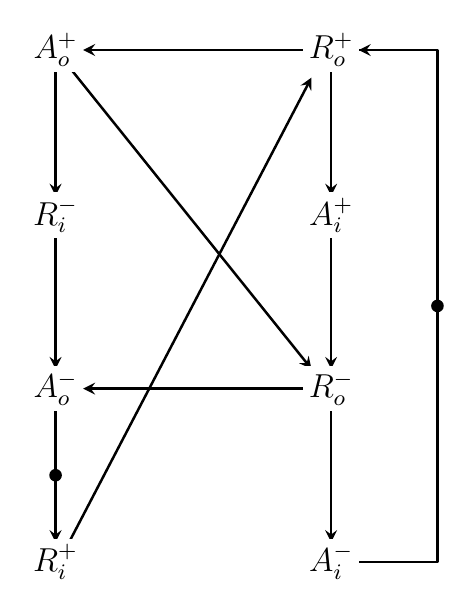
\begin{tikzpicture}[
				>=stealth,
				wire/.style={
						draw=black,
						line width=0.9pt,
						line cap=round,
						line join=round
					},
				arrow/.style={
						wire,
						->
					},
				state/.style={
						font=\large,
						fill=white,
						inner sep=2pt
					},
				dot/.style={
						circle,
						fill=black,
						inner sep=0pt,
						minimum size=0.16cm
					}
			]

			% =========================================================
			% State coordinates
			% =========================================================

			% Left column
			\coordinate (AoP) at (0,0);
			\coordinate (RiM) at (0,-2.1);
			\coordinate (AoM) at (0,-4.3);
			\coordinate (RiP) at (0,-6.5);

			% Right column
			\coordinate (RoP) at (3.5,0);
			\coordinate (AiP) at (3.5,-2.1);
			\coordinate (RoM) at (3.5,-4.3);
			\coordinate (AiM) at (3.5,-6.5);

			% =========================================================
			% Horizontal transitions
			% =========================================================

			% Ro+ -> Ao+
			\draw[arrow]
			(3.35,0) -- (0.35,0);

			% Ro- -> Ao-
			\draw[arrow]
			(3.35,-4.3) -- (0.35,-4.3);

			% =========================================================
			% Left vertical transitions
			% =========================================================

			% Ao+ -> Ri-
			\draw[arrow]
			(0,-0.20) -- (0,-1.85);

			% Ri- -> Ao-
			\draw[arrow]
			(0,-2.35) -- (0,-4.05);

			% Ao- -> Ri+
			\draw[arrow]
			(0,-4.55) -- (0,-6.25);

			% =========================================================
			% Right vertical transitions
			% =========================================================

			% Ro+ -> Ai+
			\draw[arrow]
			(3.5,-0.20) -- (3.5,-1.85);

			% Ai+ -> Ro-
			\draw[arrow]
			(3.5,-2.35) -- (3.5,-4.05);

			% Ro- -> Ai-
			\draw[arrow]
			(3.5,-4.55) -- (3.5,-6.25);

			% =========================================================
			% Diagonal transitions
			% =========================================================

			% Ao+ -> Ro-
			\draw[arrow]
			(0.12,-0.15) -- (3.25,-4.05);

			% Ri+ -> Ro+
			\draw[arrow]
			(0.12,-6.35) -- (3.25,-0.35);

			% =========================================================
			% Outer right feedback path
			% =========================================================

			% Ai- -> Ro+
			\draw[wire]
			(3.75,-6.5) -- (4.85,-6.5)
			-- (4.85,0) -- (3.85,0);

			% Arrow toward Ro+
			\draw[arrow]
			(4.35,0) -- (3.85,0);

			% =========================================================
			% Junction dots
			% =========================================================

			% Left junction
			\node[dot] at (0,-5.4) {};

			% Right junction
			\node[dot] at (4.85,-3.25) {};

			% =========================================================
			% State labels
			% =========================================================

			% Left states
			\node[state] at (AoP) {$A_o^+$};
			\node[state] at (RiM) {$R_i^-$};
			\node[state] at (AoM) {$A_o^-$};
			\node[state] at (RiP) {$R_i^+$};

			% Right states
			\node[state] at (RoP) {$R_o^+$};
			\node[state] at (AiP) {$A_i^+$};
			\node[state] at (RoM) {$R_o^-$};
			\node[state] at (AiM) {$A_i^-$};

		\end{tikzpicture}%
	}
\end{minipage}%
\hfill
\begin{minipage}[c]{0.42\linewidth}
	\centering
	\resizebox{\linewidth}{!}{%
		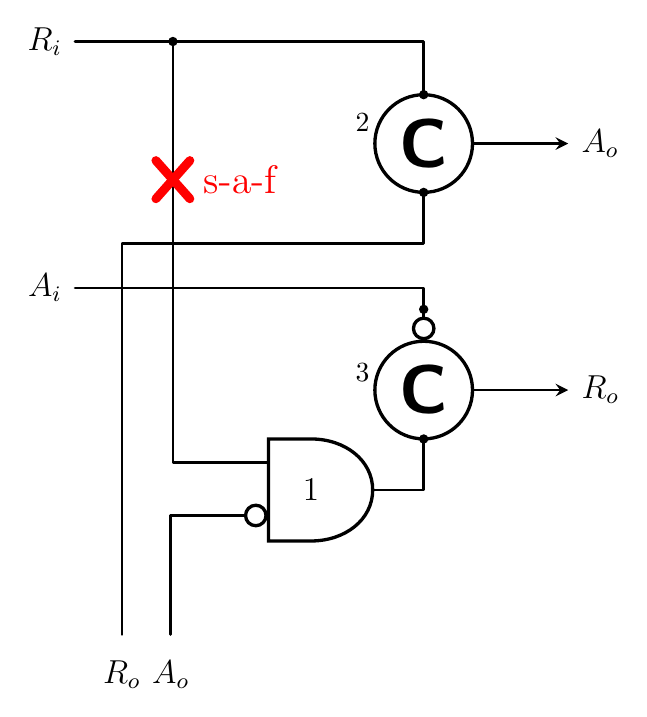
\begin{tikzpicture}[
				x=0.027cm,
				y=-0.027cm,
				wire/.style={
						draw=black,
						line width=1.0pt,
						line cap=round,
						line join=round
					},
				gate/.style={
						draw=black,
						fill=white,
						line width=1.2pt
					},
				fault/.style={
						draw=red,
						line width=3.2pt,
						line cap=round
					},
				sig/.style={
						font=\large,
						inner sep=0pt
					},
				ctext/.style={
						font=\sffamily\bfseries\fontsize{24}{26}\selectfont,
						inner sep=0pt
					},
				>=stealth
			]

			% =========================================================
			% Input Ri and branches
			% =========================================================

			% Ri -> upper C-element
			\draw[wire]
			(55,34) -- (219,34)
			-- (219,59);

			% Ri -> AND gate (upper input)
			\draw[wire]
			(101,34) -- (101,232)
			-- (146,232);

			% =========================================================
			% Input Ai
			% =========================================================

			% Ai -> lower C-element (inverted input)
			\draw[wire]
			(55,150) -- (219,150)
			-- (219,164);

			% =========================================================
			% Upper C-element feedback to Ro
			% =========================================================

			\draw[wire]
			(219,105) -- (219,129)
			-- (77,129) -- (77,313);

			% =========================================================
			% Input Ao -> AND gate (inverted)
			% =========================================================

			\draw[wire]
			(100,313) -- (100,257)
			-- (135,257);

			% =========================================================
			% AND output -> lower C-element
			% =========================================================

			\draw[wire]
			(195,245) -- (219,245)
			-- (219,221);

			% =========================================================
			% Upper C-element
			% =========================================================

			\draw[gate]
			(219,82) circle[radius=0.62cm];

			\node[ctext] at (219,82) {C};

			% Element number
			\node[
				font=\normalsize,
				anchor=east,
				inner sep=1pt
			] at (195,72) {2};

			% =========================================================
			% Lower C-element
			% =========================================================

			\draw[gate]
			(219,198) circle[radius=0.62cm];

			\node[ctext] at (219,198) {C};

			% Element number
			\node[
				font=\normalsize,
				anchor=east,
				inner sep=1pt
			] at (195,190) {3};

			% =========================================================
			% AND gate
			% =========================================================

			\draw[gate]
			(146,221) -- (166,221)
			.. controls (182,221) and (195,231) .. (195,245)
			.. controls (195,259) and (182,269) .. (166,269)
			-- (146,269) -- cycle;

			% Gate number
			\node[
				font=\large,
				inner sep=0pt
			] at (166,245) {1};

			% =========================================================
			% Inversion bubble: Ao -> AND
			% =========================================================

			\draw[gate]
			(140,257) circle[radius=0.13cm];

			% =========================================================
			% Inversion bubble: Ai -> lower C
			% =========================================================

			\draw[gate]
			(219,169) circle[radius=0.13cm];

			% =========================================================
			% Output Ao
			% =========================================================

			\draw[wire,->]
			(242,82) -- (287,82);

			% =========================================================
			% Output Ro
			% =========================================================

			\draw[wire,->]
			(242,198) -- (287,198);

			% =========================================================
			% Junction dots
			% =========================================================

			\foreach \p in {
					(101,34),
					(219,59),
					(219,105),
					(219,160),
					(219,221)
				}{
					\fill[black] \p circle[radius=1.7pt];
				}

			% =========================================================
			% Stuck-at-f fault marker
			% =========================================================

			% Red X on Ri branch
			\draw[fault]
			(93,90) -- (109,108);

			\draw[fault]
			(109,90) -- (93,108);

			% Fault label
			\node[
				font=\Large,
				text=red,
				anchor=west,
				inner sep=0pt
			] at (115,99) {s-a-f};

			% =========================================================
			% Input labels
			% =========================================================

			\node[sig,anchor=east] at (49,34) {$R_i$};
			\node[sig,anchor=east] at (49,150) {$A_i$};

			% =========================================================
			% Output labels
			% =========================================================

			\node[sig,anchor=west] at (293,82) {$A_o$};
			\node[sig,anchor=west] at (293,198) {$R_o$};

			% =========================================================
			% Lower signal labels
			% =========================================================

			\node[sig] at (77,332) {$R_o$};
			\node[sig] at (100,332) {$A_o$};

		\end{tikzpicture}%
	}
\end{minipage}

\end{problem}

\begin{solution}
	\noindent Circuit equations (C = Muller C-element):
	\[
		A_o = C(R_i,\ R_o),\qquad R_o = C\big(\overline{A_i},\ R_i\cdot\overline{A_o}\big).
	\]
	Initial state: \(R_i = A_i = A_o = R_o = 0\), so the AND gate output is \(0\) and the next expected transition is \(R_i^+ \rightarrow R_o^+\).
	The fault is on the \(R_i\) input of the AND gate (1).

	\myspace

	\noindent\textbf{Stuck-at-0 \(\Rightarrow\) Inhibited transition.}
	The AND output is always \(0\), so C-element 3 can never set \(R_o = 1\).
	After \(R_i^+\), the transition \(R_o^+\) never fires, so \(A_o^+\) (needs \(R_o = 1\)) never fires either and the circuit deadlocks.

	\myspace

	\noindent\textbf{Stuck-at-1 \(\Rightarrow\) Premature transition.}
	The AND output becomes \(\overline{A_o} = 1\). Together with \(\overline{A_i} = 1\), both inputs of C-element 3 are \(1\) in the initial state,
	so \(R_o^+\) fires immediately \emph{before} \(R_i^+\) arrives, violating the order \(R_i^+ \rightarrow R_o^+\) of the STG.
\end{solution}
% ================================================================================ %

\end{document}
